\documentclass{beamer}
\usepackage{graphicx}
\usepackage{paralist}
\usepackage{outlines}

\title{TOPIC}
\author{Mendocino College - Digital Image Manipulation with Photoshop}
\titlegraphic{\vspace{-10mm}
\includegraphics[width = .9\textwidth]{images/photoshop.jpg}} 
\date{\vspace{-5em}} 


\mode <presentation>
\usetheme{Warsaw}
\usecolortheme{default}

\setbeamerfont{footline}{size=\fontsize{5}{8}\selectfont}

\definecolor{darkred}{rgb}{20,0,0}
\definecolor{darkgreen}{RGB}{40,110,20}
\definecolor{darkpurple}{RGB}{30,0,30}
\definecolor{chardonnay}{RGB}{255, 255, 204}

\setbeamercolor*{palette primary}{fg=white, bg=darkgreen}

\setbeamersize{text margin left=0pt, text margin right=0pt}


\begin{document}
	{
		\setbeamertemplate{footline}{} 
		\setbeamertemplate{headline}{} 
		\begin{frame}
			\vspace{-35pt}
			\maketitle
		\end{frame}
	}
		
		
\section{What is a Resume?}

\subsection{What is a Resume?}		

	\begin{frame}
		\frametitle{What is a Resume?}
		\begin{outline}
			\1 A resume is a formal document that provides an overview of your professional qualifications, including your relevant work experience, skills, education, and notable accomplishments. 
			
			\1 Usually paired with a cover letter, a resume helps you demonstrate your abilities and convince employers you’re qualified and hireable.
			
			\1 The purpose of a resume is to show employers you’re qualified for a position and convince them to offer you an interview.
			
			\2 Called a "CV" outside of America, and with graduate schools.
			
			\1 Many job seekers wrongly assume their resume should provide a full overview of their professional history.
			
			\2 Instead, think of your resume as an advertisement of yourself. 
			
			\1 Your resume should only emphasize your most relevant experience and skills, and highlight your most notable strengths and accomplishments.
		\end{outline}
	\end{frame}

\subsection{Resume Topics}
\begin{frame}
	\frametitle{Topics to Include on your Resume}
	\begin{outline}
		\1 Contact details: 
		\2 When writing your contact information on your resume, include your first and last name, phone number, and email address. 
		\2 Additionally, you can add your LinkedIn profile. 
		\2 List your city if you want to show you live near where the company is located, but your mailing address isn’t necessary.
		\1 Introduction: 
		\2 A concise overview of your professional background and key qualifications. 
		\2 Your introduction can be in the form of a resume summary or resume objective.
		\2 A resume summary is a 1-5 sentence introduction that highlights your most relevant career experience, skills, and achievements. 
		\3 The first sentence should always include your biggest professional selling points.
		\2 An objective on a resume is an introduction that addresses a specific job ad, acting as a career mission statement by introducing the skills and qualifications you can bring to a position.
	\end{outline}
\end{frame}

\begin{frame}
	\frametitle{Topics to include on your Resume}
	\begin{outline}
		\1 Educational Background: 
		\2 Your resume’s education section can include your school name(s), highest degree earned, majors and minors. 
		\2 Additionally, you can add your GPA (if it’s greater than 3.8), Dean’s list (if you’ve been on it), and relevant coursework if you lack experience or it’s related to the position.
		\1 Work History:  
		\2 List any relevant work experience you have. 
		\2 Include your title, the company you worked for, years (or months) worked, and bullet points outlining your key responsibilities and notable accomplishments.
		\1 Relevant Skills: 
		\2 Include skills on your resume that are relevant to the position. 
		\2 Be sure to use a strong mix of hard skills and soft skills to demonstrate that you’re a well-rounded candidate.
	\end{outline}
\end{frame}

\subsection{Classic Example}		
\begin{frame}
	\frametitle{Example of a Classic Resume}
	\vspace{-5pt}
	\begin{center}
		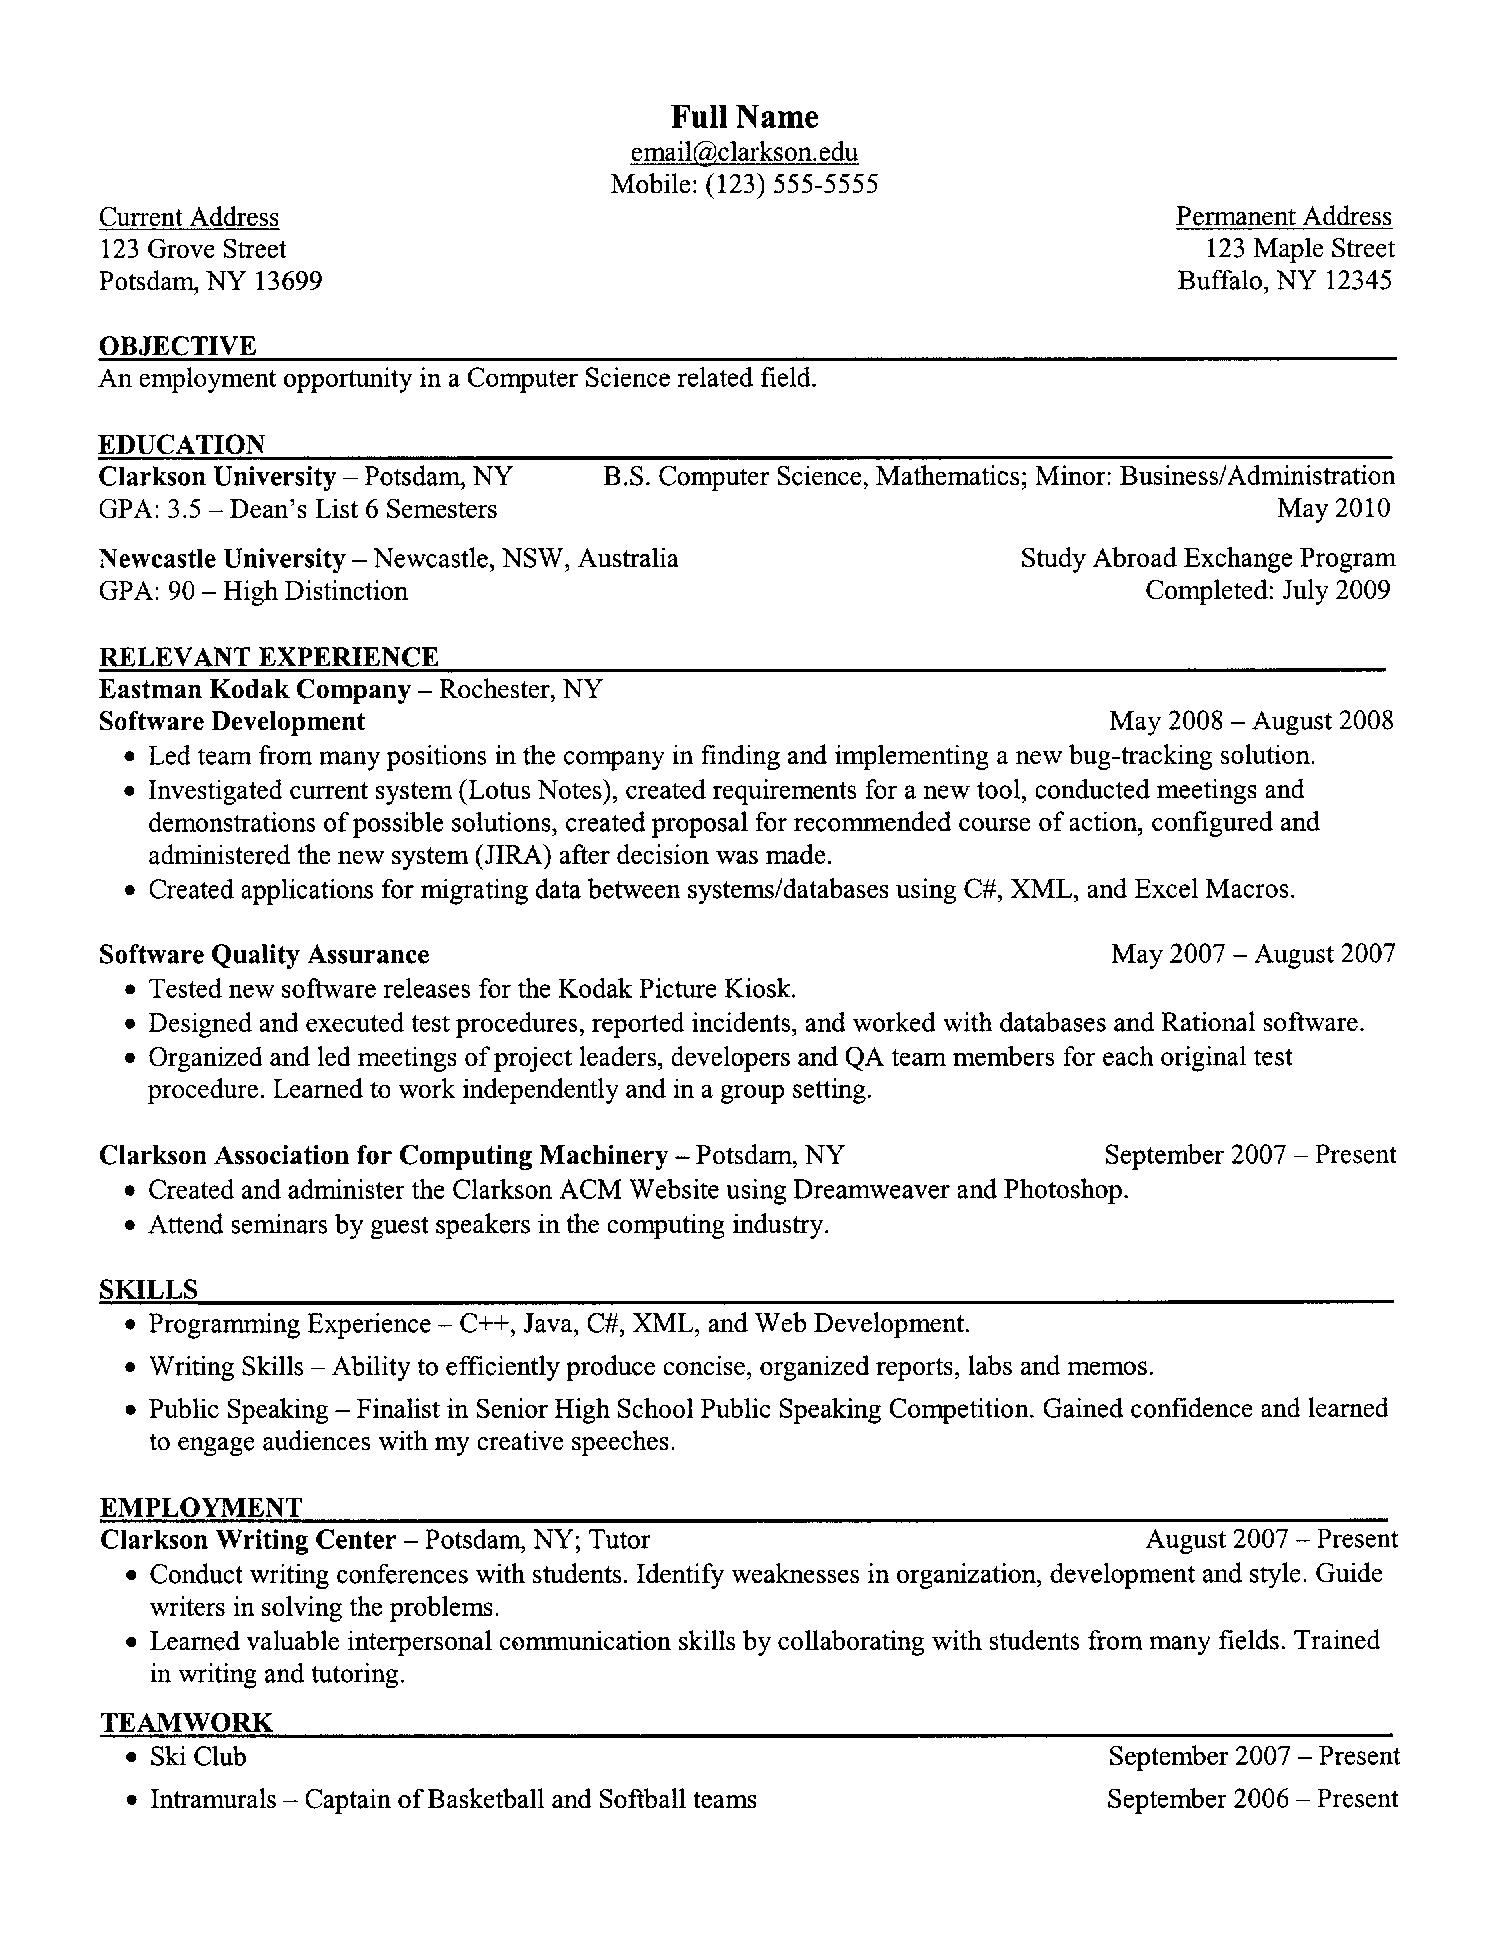
\includegraphics[width=0.45\textwidth]{images/Resume-Sample-7.jpg}
	\end{center}
\end{frame}

\section{Writing your resume}
	\subsection{How to write your Resume}
\begin{frame}
	\frametitle{How to write your Resume}
	\begin{outline}
		\1 To write a strong resume, scan through the job listing for the position you want to fill. 
		\2 Typically, hiring managers include the skills, responsibilities, and traits that they want candidates to possess directly in the job description. 
		\2 Showcase these qualities on your resume to demonstrate you’re an ideal fit.
		\1 Focus on your skills and abilities rather than your career progression.
		\2 Categorizes your professional and educational accomplishments according to the skills they demonstrates.
		\1 A good resume is the first part of your application that any hiring manager will see.
		\2 It is important that it conveys your qualifications accurately and convincingly.
		\2 It is based on this information, they can make an informed decision about whether or not they want to interview and eventually hire you.
		\1 Dont include your street address, only the city and state.
		\1 Do not have a picture of your face.
		\1 Less is More
	\end{outline}
\end{frame}

\subsection{Length of Resume}
	\begin{frame}
	\frametitle{How long should a resume be?}
	\begin{outline}
		\1 Always keep your resume to 1-page
		\1 It must be concise, accurate, and compelling.
		\1 A second additional page to your resume is only for when the potential employer is interested enough to continue looking into you.
		\2 Only include additional information that you want a future employer to know about you.
		\2 It should have another purpose, such as a second page to your portfolio.
		\2 If you do not have a good 1-page resume, then a second page does not even matter.
	\end{outline}
\end{frame}

\subsection{2nd Resume Page Example}		
	\begin{frame}
		\frametitle{Example of my resume's second page}
		\vspace{-5pt}
		\begin{center}
			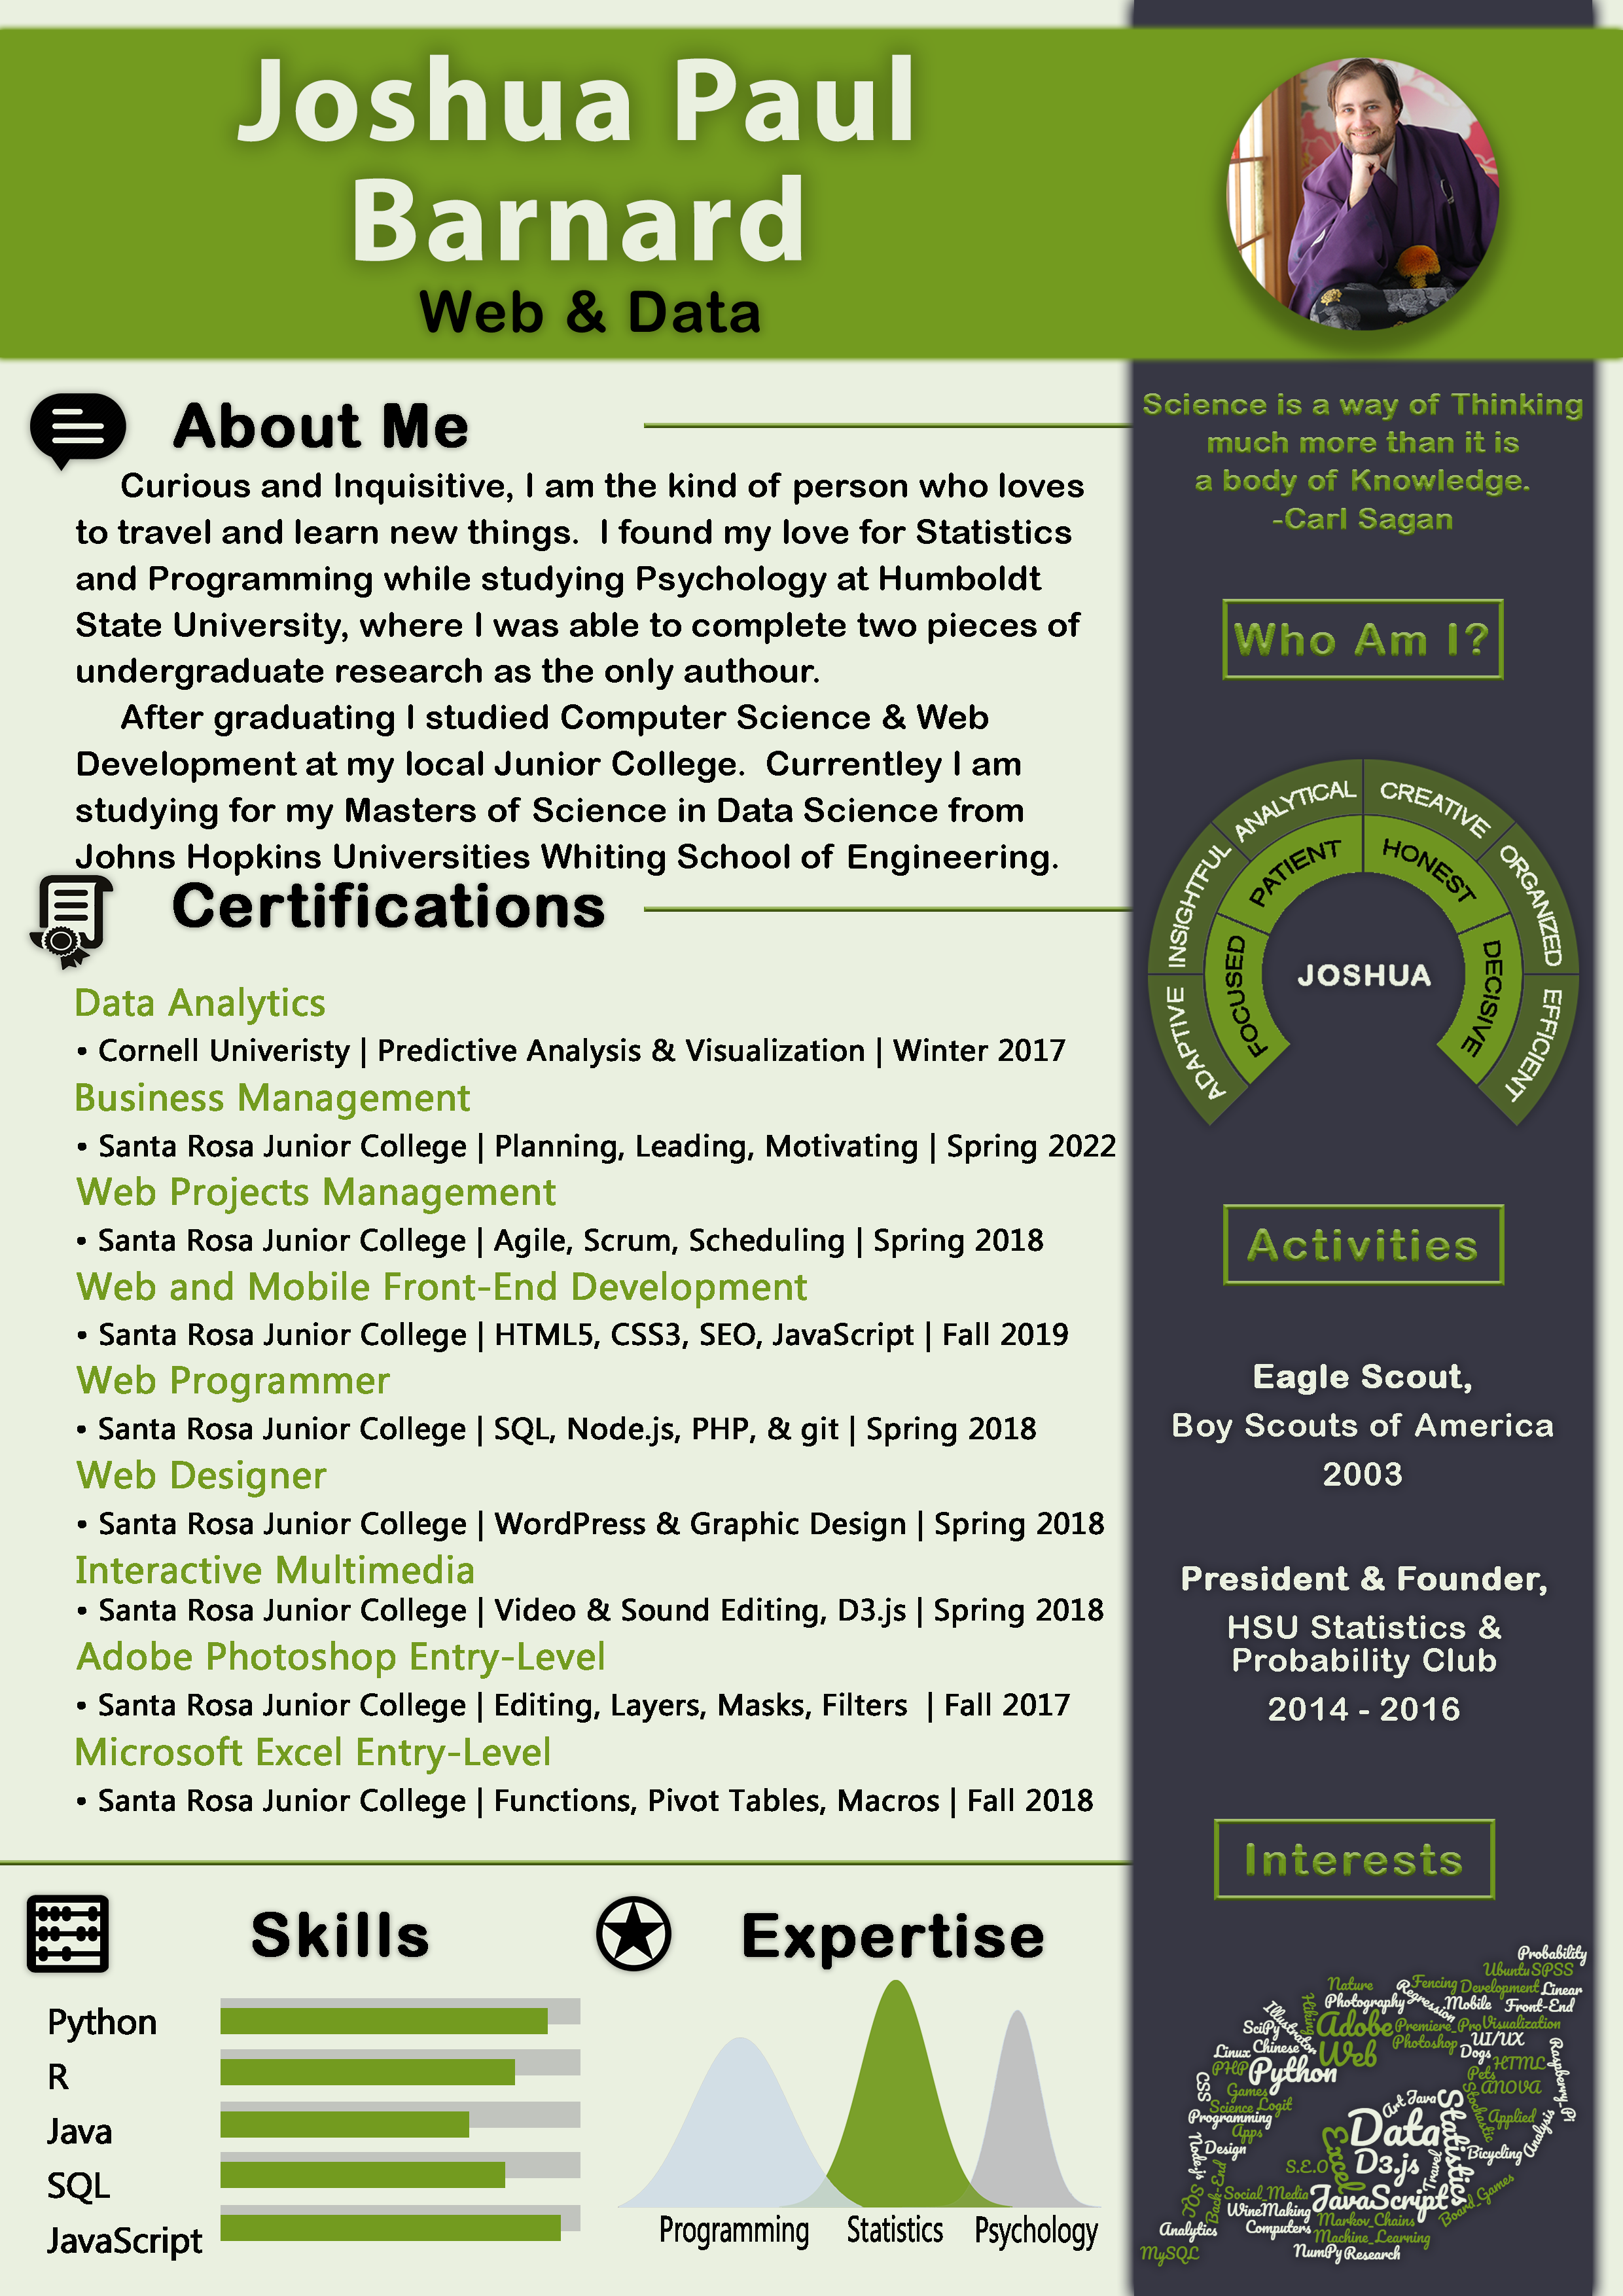
\includegraphics[width=0.4\textwidth]{images/Joshua_Paul_Barnard-second_page.png}
		\end{center}
	\end{frame}


\section{Resources}
\subsection{Additional Resources for Resumes}		
	\begin{frame}
		\frametitle{Additional Resources for Resumes}
		\begin{outline}
			\1 What is a Resume? Definition and Purpose
			\2  By:    Conrad Benz 
			\2  Date:  September 18, 2022
			\2  Pages: 23
			\2 https://resumegenius.com/blog/resume-help/what-is-a-resume
			\1 5 Things You Don't Need on Your Resume Anymore
			\2  By:      Don Georgevich
			\2  Length:  15:37
			\2 https://www.youtube.com/watch?v=8\_ImWB1qMf8
		\end{outline}
	\end{frame}

	
\end{document}